\documentclass[a4paper,11pt]{book}
%\documentclass[a4paper,twoside,11pt,titlepage]{book}
\usepackage{listings}
\usepackage[utf8]{inputenc}
\usepackage[spanish]{babel}

\usepackage[acronym, numberedsection=autolabel, entrycounter]{glossaries} %
\usepackage{amsmath} 
\usepackage{nameref}
%\usepackage{titlesec}
%\usepackage{pailatino}
\usepackage{appendix}
\decimalpoint
\usepackage{dcolumn}
\newcolumntype{.}{D{.}{\esperiod}{-1}}
\makeatletter
\addto\shorthandsspanish{\let\esperiod\es@period@code}
\makeatother


%\usepackage[chapter]{algorithm}
\RequirePackage{verbatim}
%\RequirePackage[Glenn]{fncychap}
\usepackage{fancyhdr}
\usepackage{graphicx}
\usepackage{afterpage}
\usepackage{xspace}
\usepackage{longtable}

\usepackage[pdfborder={000}]{hyperref} %referencia

% ********************************************************************
% Re-usable information
% ********************************************************************
\newcommand{\myTitle}{Desarrollo de un prototipo de motor de búsqueda que incorpore técnicas bibliométricas para mejorar la recuperación\xspace}
\newcommand{\myDegree}{Master Universitario en Ingeniería Informática\xspace}
\newcommand{\myName}{Aythami Estévez Olivas\xspace}
\newcommand{\myProf}{Juan Manuel Fernández Luna\xspace}
\newcommand{\myOtherProf}{Nombre Apllido1 Apellido2 (tutor2)\xspace}
%\newcommand{\mySupervisor}{Put name here\xspace}
\newcommand{\myFaculty}{Escuela Técnica Superior de Ingenierías Informática y de
Telecomunicación\xspace}
\newcommand{\myFacultyShort}{E.T.S.I.I.T.\xspace}
\newcommand{\myDepartment}{Departamento de Ciencias de la Computación e Inteligencia Artificial\xspace}
\newcommand{\myUni}{\protect{Universidad de Granada}\xspace}
\newcommand{\myLocation}{Granada\xspace}
\newcommand{\myTime}{\today\xspace}
\newcommand{\myVersion}{Version 0.1\xspace}


\hypersetup{
urlcolor=blue,
pdfauthor = {\myName (aythae (at) correo (punto) ugr (punto) es)},
pdftitle = {\myTitle},
pdfsubject = {},
pdfkeywords = {palabra_clave1, palabra_clave2, palabra_clave3, ...},
pdfcreator = {LaTeX con el paquete pdflatex},
pdfproducer = {pdflatex}
}

%\hyphenation{}


%\usepackage{doxygen/doxygen}
%\usepackage{pdfpages}
\usepackage{url}
\usepackage{colortbl,longtable}
\usepackage[stable]{footmisc}
%\usepackage{index}

%\makeindex
%\usepackage[style=long, cols=2,border=plain,toc=true,number=none]{glossary}
% \makeglossary

% Definición de comandos que me son tiles:
%\renewcommand{\indexname}{Índice alfabético}
%\renewcommand{\glossaryname}{Glosario}
\renewcommand{\appendixname}{Anexos}
\renewcommand{\appendixtocname}{Anexos}
\renewcommand{\appendixpagename}{Anexos}
\pagestyle{fancy}
\fancyhf{}
\fancyhead[LO]{\leftmark}
\fancyhead[RE]{\rightmark}
\fancyhead[RO,LE]{\textbf{\thepage}}
\renewcommand{\chaptermark}[1]{\markboth{\textbf{#1}}{}}
\renewcommand{\sectionmark}[1]{\markright{\textbf{\thesection. #1}}}

\setlength{\headheight}{1.5\headheight}

\newcommand{\HRule}{\rule{\linewidth}{0.5mm}}
%Definimos los tipos teorema, ejemplo y definición podremos usar estos tipos
%simplemente poniendo \begin{teorema} \end{teorema} ...
\newtheorem{teorema}{Teorema}[chapter]
\newtheorem{ejemplo}{Ejemplo}[chapter]
\newtheorem{definicion}{Definición}[chapter]

\definecolor{gray97}{gray}{.97}
\definecolor{gray75}{gray}{.75}
\definecolor{gray45}{gray}{.45}
\definecolor{gray30}{gray}{.94}

\lstset{ frame=Ltb,
     framerule=0.5pt,
     aboveskip=0.5cm,
     framextopmargin=3pt,
     framexbottommargin=3pt,
     framexleftmargin=0.1cm,
     framesep=0pt,
     rulesep=.4pt,
     backgroundcolor=\color{gray97},
     rulesepcolor=\color{black},
     %
     stringstyle=\ttfamily,
     showstringspaces = false,
     basicstyle=\s\left( criptsize\ttfamily,
     commentstyle=\color{gray45},
     keywordstyle=\bfseries,
     %
     numbers=left,
     numbersep=6pt,
     numberstyle=\tiny,
     numberfirstline = false,
     breaklines=true,
   }
 
% minimizar fragmentado de listados
\lstnewenvironment{listing}[1][]
   {\lstset{#1}\pagebreak[0]}{\pagebreak[0]}

\lstdefinestyle{CodigoC}
   {
	basicstyle=\scriptsize,
	frame=single,
	language=C,
	numbers=left
   }
\lstdefinestyle{CodigoC++}
   {
	basicstyle=\small,
	frame=single,
	backgroundcolor=\color{gray30},
	language=C++,
	numbers=left
   }

 
\lstdefinestyle{Consola}
   {basicstyle=\scriptsize\bf\ttfamily,
    backgroundcolor=\color{gray30},
    frame=single,
    numbers=none
   }


\newcommand{\bigrule}{\titlerule[0.5mm]}


%Para conseguir que en las páginas en blanco no ponga cabecerass
\makeatletter
\def\clearpage{%
  \ifvmode
    \ifnum \@dbltopnum =\m@ne
      \ifdim \pagetotal <\topskip
        \hbox{}
      \fi
    \fi
  \fi
  \newpage
  \thispagestyle{empty}
  \write\m@ne{}
  \vbox{}
  \penalty -\@Mi
}
\makeatother

\renewcommand*{\glsentrycounterlabel}{}
\makenoidxglossaries
\newglossaryentry{latex}
{
	name=latex,
	description={Is a mark up language specially suited for 
		scientific documents}
}
\newacronym{RI}{RI}{Recuperación de Información}

\usepackage{pdfpages}
\begin{document}
\begin{titlepage}
 
 
\newlength{\centeroffset}
\setlength{\centeroffset}{-0.5\oddsidemargin}
\addtolength{\centeroffset}{0.5\evensidemargin}
\thispagestyle{empty}

\noindent\hspace*{\centeroffset}\begin{minipage}{\textwidth}

\centering

\includegraphics[width=0.9\textwidth]{imagenes/logo_ugr.jpg}\\[1.4cm]

\textsc{ \Large TRABAJO FIN DE MÁSTER\\[0.2cm]}
\textsc{ MÁSTER UNIVERSITARIO EN INGENIERÍA INFORMÁTICA}\\[1cm]
% Upper part of the page
% 
% Title
{\LARGE\bfseries \myTitle\\
}
%\noindent\rule[-1ex]{\textwidth}{3pt}\\[3.5ex]
%{\large\bfseries Subtitulo del Proyecto}
\end{minipage}

\vspace{2.5cm}
\noindent\hspace*{\centeroffset}\begin{minipage}{\textwidth}
\centering

\textbf{Autor}\\ \myName\\[2.5ex]
\textbf{Directores}\\
\myProf\\[2cm]

\includegraphics[width=0.3\textwidth]{imagenes/etsiit_logo.png}\\[0.1cm]
\textsc{Escuela Técnica Superior de Ingenierías Informática y de Telecomunicación}\\
\textsc{---}\\
\myLocation, \myTime
\end{minipage}
%\addtolength{\textwidth}{\centeroffset}
%\vspace{\stretch{2}}
\end{titlepage}



%\chapter*{}
%\thispagestyle{empty}
%\cleardoublepage

%\thispagestyle{empty}

%\begin{titlepage}
 
 
\setlength{\centeroffset}{-0.5\oddsidemargin}
\addtolength{\centeroffset}{0.5\evensidemargin}
\thispagestyle{empty}

\noindent\hspace*{\centeroffset}\begin{minipage}{\textwidth}

\centering
%
\includegraphics[width=0.9\textwidth]{imagenes/logo_ugr.jpg}\\[1.4cm]

%\textsc{ \Large PROYECTO FIN DE CARRERA\\[0.2cm]}
%\textsc{ INGENIERÍA EN INFORMÁTICA}\\[1cm]
% Upper part of the page
% 

 \vspace{3.3cm}

%si el proyecto tiene logo poner aquí

\includegraphics{imagenes/logo.png} 
 \vspace{0.5cm}

% Title

{\Huge\bfseries Título del proyecto\\
}
\noindent\rule[-1ex]{\textwidth}{3pt}\\[3.5ex]
{\large\bfseries Subtítulo del proyecto.\\[4cm]}
\end{minipage}

\vspace{2.5cm}
\noindent\hspace*{\centeroffset}\begin{minipage}{\textwidth}
\centering

\textbf{Autor}\\ {Nombre Apellido1 Apellido2 (alumno)}\\[2.5ex]
\textbf{Directores}\\
{Nombre Apellido1 Apellido2 (tutor1)\\
Nombre Apellido1 Apellido2 (tutor2)}\\[2cm]
%
\includegraphics[width=0.15\textwidth]{imagenes/tstc.png}\\[0.1cm]
%\textsc{Departamento de Teoría de la Señal, Telemática y Comunicaciones}\\
%\textsc{---}\\
%Granada, mes de 201
\end{minipage}
%\addtolength{\textwidth}{\centeroffset}
\vspace{\stretch{2}}

 
\end{titlepage}






\cleardoublepage
\thispagestyle{empty}

\begin{center}
{\large\bfseries \myTitle}\\
\end{center}
\begin{center}
\myName\\
\end{center}

%\vspace{0.7cm}
\noindent{\textbf{Palabras clave}: Recuperación de información, Bibliometría, \acrlong{ES}}\\

\vspace{0.7cm}
\noindent{\textbf{Resumen}}\\

Todos utilizamos motores de búsqueda en nuestra vida diaria y cada vez somos más dependientes de los mismos debido al exponencial incremento de información que se genera diariamente en los últimos tiempos. Esto hace cada vez más importante la mejora de los sistemas de búsqueda, para que sean capaces de priorizar y ayudarnos a encontrar la información que necesitamos.

En el mundo científico también ocurre esto, un investigador necesita la ayuda de algún sistema de recuperación de información para poder mantenerse al día en su rama de investigación. Por ello este proyecto propone un modelo alternativo de sistema de búsqueda, que tenga en cuenta medidas bibliométricas características de los artículos científicos, como el número de citas o el índice h, para mejorar la recuperación.

En concreto, el sistema planteado combinará la información bibliométrica con los resultados de búsquedas por contenido tradicionales de distintos modos. Este sistema se ha desarrollado como una aplicación web distribuida, que se servirá de una interfaz de usuario para realizar búsquedas por autores o artículos y comparar los resultados obtenidos con las distintas combinaciones.

Para desarrollar dicho sistema se ha empleado una metodología de desarrollo ágil que permite desarrollar de forma rápida e iterativa.


\cleardoublepage


\thispagestyle{empty}
%
%
\begin{center}
{\large\bfseries Project Title: Project Subtitle}\\
\end{center}
\begin{center}
First name, Family name (student)\\
\end{center}

%\vspace{0.7cm}
\noindent{\textbf{Keywords}: Keyword1, Keyword2, Keyword3, ....}\\

\vspace{0.7cm}
\noindent{\textbf{Abstract}}\\

Write here the abstract in English.
%
\chapter*{}
\thispagestyle{empty}

\noindent\rule[-1ex]{\textwidth}{2pt}\\[4.5ex]

Yo, \textbf{\myName}, alumno de la titulación \myDegree de la \textbf{\myFaculty de la \myUni}, con DNI 70918176E, autorizo la
ubicación de la siguiente copia de mi Trabajo Fin de Máster en la biblioteca del centro para que pueda ser
consultada por las personas que lo deseen.

\vspace{6cm}

\noindent Fdo: \myName

\vspace{2cm}

\begin{flushright}
\myLocation a \myTime.
\end{flushright}


\chapter*{}
\thispagestyle{empty}

\noindent\rule[-1ex]{\textwidth}{2pt}\\[4.5ex]

D. \textbf{\myProf}, Profesor del Área de Ciencias de la Computación e Inteligencia Artificial del \myDepartment
 de la Universidad de Granada.

\vspace{0.5cm}

\textbf{Informa:}

\vspace{0.5cm}

Que el presente trabajo, titulado \textit{\textbf{\myTitle}},
ha sido realizado bajo su supervisión por \textbf{\myName}, y autorizo la defensa de dicho trabajo ante el tribunal
que corresponda.

\vspace{0.5cm}

Y para que conste, expiden y firman el presente informe en Granada a \myTime.

\vspace{1cm}

\textbf{El director:}

\vspace{5cm}

\noindent \textbf{\myProf }
%
%\chapter*{Agradecimientos}
%\thispagestyle{empty}
%
%       \vspace{1cm}


%Poner aquí agradecimientos...


\frontmatter
\tableofcontents
\listoffigures
\listoftables
%
\mainmatter
\setlength{\parskip}{5pt}

\chapter{Introducción}
\section{Motivación}

A día de hoy usamos constantemente buscadores: web como Google o Bing, de ficheros como los integrados en todos los sistemas de ficheros modernos o de contenido como puede ser una búsqueda de algún término en un \acrshort{PDF} como este. Todo buscador es conocido desde un punto de vista más técnico como un \textbf{Sistemas de \acrfull{RI}}. 

Tradicionalmente estos sistemas realizan una búsqueda por contenido, si buscamos una palabra o término de búsqueda concreto en Google, este retorna páginas relevantes que contentan dicha palabra. 

Esto también funciona así para la recuperación de artículos científicos, pero en este caso los artículos científicos disponen de algunas medidas asociadas como el número de citas que pueden ser interesantes para determinar la relevancia de un artículo. Se puede entender que si un par de artículos contienen un término de búsqueda, él que sea más citado parece, a \textit{priori}, más relevante, ya que la propia comunidad científica lo menciona con mayor frecuencia. Dichas métricas asociadas a la literatura científica se conocen como \textbf{medidas bibliométricas}.

Este proyecto pretende explorar las posibilidades de estas medidas para mejorar los procesos de recuperación de información.

Durante la asignatura del máster \acrfull{GIW}, se vieron algunas pinceladas de las herramientas empleadas para llevar a cabo sistemas de \acrlong{RI}, así como su base teórica. Esto me llamó realmente la atención, ya que todos utilizamos diariamente sistemas de búsqueda, pero no tenía ni idea de como se podía implementar uno. A pesar de haber desarrollado un pequeño sistema como parte de sus prácticas me quedé con la ganas de ver un sistema "más real", desarrollado con herramientas más potentes. Este es el principal motivo por el que me decanté a la realización de este proyecto, a nivel personal me gustaría poder llenar esta curiosidad con el desarrollo del presente trabajo.

\section{Objetivos}

En este apartado recogeré de manera sintetizada los objetivos del proyecto, lo cual ayudará a comprender la funcionalidad del sistema a desarrollar así como definir su alcance. El objetivo principal es \textbf{desarrollar un Sistema de \acrlong{RI} que incorpore medidas bibliométricas como mejora a la recuperación clásica}. Junto a este objetivo también tenemos 

%\section{Objetivos generales}
\begin{itemize}

	
	\item \textbf{Descomponer el sistema de \acrshort{RI}}: Observando los diversos sistemas reales de recuperación de información científica que he analizado, como Google Scholar o Scopus, la gran mayoría dividen la búsqueda en búsqueda de autores y de artículos en sí. Ya que estos son dos tipos de datos diferenciados (aunque relacionados profundamente) e intuitivamente, se comprende que un sistema de RI funcionará mejor si los datos del mismo son homogéneos. Por ello el sistema a desarrollar dispondrá de dos partes una búsqueda de autores y otra de artículos.
	
	\item \textbf{Desarrollar un sistema que sea usable}: Muchos de los enfoques que he visto durante mi proceso de documentación no pasan de modelos teóricos, prototipos o sistemas en los que la usabilidad y la orientación al usuario brillan por su ausencia. Aunque este no sea el punto objetivo principal del sistema, me parece muy importante que se tenga en cuenta al usuario durante todo el proceso de desarrollo, ya que un sistema puede ser increíble pero si los usuarios no lo entienden o no le saben sacar partido no sirve de nada. Por ello, pretendo diseñar una interfaz de usuario que sea simple de usar, empleando metáforas y componentes ampliamente conocidos por los usuarios.

\end{itemize}


\section{Organización de la memoria}

Esta memoria detallará el desarrollo del proyecto desde su comienzo hasta su conclusión y cuenta con los siguientes apartados:
\begin{itemize}
	\item El siguiente capítulo versa sobre los aspectos de la \textbf{planificación} del proyecto, desde una perspectiva temporal, económica, de recursos y metodológica.
	\item Tras esto se definirá el \textbf{contexto} del trabajo, dando antecedentes, definiendo los principales conceptos teóricos y analizando el estado del arte.
	\item En el capítulo \textbf{análisis} se planteará el proyecto a desarrollar, ayudándose de historias de usuario para definir la funcionalidad del sistema creado.
	\item Este planteamiento se refinará y detallará en el \textbf{diseño}, centrándose en los datos y arquitectura del sistema.
	\item El grueso de la memoria está constituido por el \textbf{desarrollo}, donde se han apuntado los principales aspectos del mismo, siguiendo una estructura de \textit{sprints}, así como la aclaración de la arquitectura del sistema final.
	\item Para finalizar el contenido principal, el apartado de \textbf{conclusiones y trabajos futuros} recoge algunas reflexiones personales y sobre los resultados del proyecto, incluyendo algunos posibles caminos futuros de ampliación del mismo.
	\item Tras esto se pueden encontrar la \textbf{bibliografía}, así como los anexos \textbf{glosario}, \textbf{lista de acrónimos} y un \textbf{manual técnico de uso} donde se detalla la arquitectura final con instrucciones de instalación y despliegue.
\end{itemize}




\chapter{Objetivos}

En este capítulo recogeré de manera sintetizada los objetivos del proyecto, lo cual ayudará a comprender la funcionalidad del sistema a desarrollar así como definir su alcance.

%\section{Objetivos generales}
\begin{itemize}
	\item \textbf{Obtención de artículos o \textit{papers} de autores de la escuela}: como colección de datos del sistema \acrshort{RI} a desarrollar se ha decidido utilizar el conjunto de todos los trabajos de autores de la \myFaculty, ya que la familiaridad de los datos permite analizar si los resultados obtenidos tienen sentido. Esto puede servir para comprender relaciones como que un par de autores del mismo grupo de investigación o departamento aparezcan juntos en los resultados, muy relacionado con esto se encuentra el siguiente objetivo.
	\item \textbf{Evaluar si la mejora producida al aplicar medidas bibliométricas al sistema}: El objetivo anterior favorece que esta evaluación se pueda llevar a cabo, aunque esta no es una tarea sencilla. La evaluación de sistemas \acrshort{RI} se suele llevar a cabo mediante colecciones de prueba donde existe un conjunto de documentos, un conjunto de consultas y un conjunto de resultados que deberían de retornar las mismas  \cite{RI_Evaluation}. Al crear un sistema nuevo con una colección de documentos no utilizada no podemos comparar los resultados obtenidos con los que se esperarían, este problema se debe a la relatividad del concepto de relevancia. Por ello las colecciones de pruebas suelen incluir valoraciones de relevancia de expertos en la materia.
	\item \textbf{Desarrollar un sistema que sea usable}: Muchos de los enfoques que he visto durante mi proceso de documentación no pasan de modelos teóricos, prototipos o sistemas en los que la usabilidad y la orientación al usuario brillan por su ausencia. Aunque este no sea el punto objetivo principal del sistema me parece muy importante que se tenga en cuenta al usuario durante todo el proceso de desarrollo, ya que un sistema puede ser increíble pero si los usuarios no lo entienden o no le saben sacar partido no sirve de nada. Por ello pretendo diseñar una interfaz de usuario que sea simple de usar y emplee metáforas y componentes ampliamente conocidos por los usuarios.
	\item \textbf{Conocer y emplear tecnologías punteras en el ámbito de la \acrshort{RI}}: durante la asignatura del máster \acrfull{GIW} se vieron algunas pinceladas de las herramientas empleadas para llevar a cabo estos sistemas así como su base teórica. Esto me llamo realmente la atención ya que todos utilizamos sistemas de búsqueda, pero no tenía ni idea de como se podía implementar uno. A pesar de haber desarrollado un pequeño sistema como parte de sus prácticas me quedé con la ganas de ver herramientas más potentes. Este es el principal motivo por el que me decanté a la realización de este proyecto, a nivel personal me gustaría cumplir con creces este objetivo.
\end{itemize}

\chapter{Planificación}

\section{Gestión de recursos}
En este apartado describiré brevemente los recursos utilizados para llevar a cabo este proyecto tiendo en cuenta personal, hardware y software.

\subsection{Personal}
El único recurso humano que ha contribuido a la realización del proyecto soy yo mismo actuando como los diversos roles que llevan acabo el proceso de desarrollo de un proyecto de estas características.

\subsection{Hardware}
Respecto al hardware utilizado para este \acrshort{TFM} solo he requerido mi ordenador portátil personal, cuyas características se destacan en la siguiente tabla:

\begin{table} [h!]
\centering
\begin{tabular}{c c}
	\hline
	CPU & Intel \textregistered  Core \texttrademark  i7-4700MQ CPU @ 2.40GHz x 8\\
	RAM & 8 GB RAM DDR3\\
	Almacenamiento & HDD 750 GB (5400 RPM)\\
	\hline
\end{tabular}
	\caption{Especificaciones del equipo utilizado}
\end{table}

Esto ha bastado para el desarrollo, pero seria necesario conseguir un servidor en condiciones para llegar a poner en producción el sistema. Tampoco sería necesario nada muy potente ya que incluso en mi propio ordenador los tiempos empleados en la búsqueda son bastante aceptables.

\subsection{Software}
Se han empleado utilidades de software libre en la totalidad del proyecto. Aquí enumerare el principal software empleado y su función primordial, para una descripción más detalladas de las herramientas empleadas ver el capítulo \nameref{ch:herramientas}:

\begin{itemize}
	\item \textbf{Debian}: \acrfull{SO}.
	\item \textbf{Python}: Lenguaje de programación usado en las primeras fases del proyecto y en servidor \gls{backend} \glsrefentry{backend}.
	\item \textbf{JavaScript}: Lenguaje de programación interpretado en el que se ha escrito el \gls{frontend} \glsrefentry{frontend}.
	\item \textbf{Elasticsearch}: Servidor de búsqueda.
	\item \textbf{MongoDB}: Base de datos NoSQL.
	\item \textbf{React}:  \Gls{framework} para el desarrollo de interfaces de usuario.
	\item \textbf{Searchkit}: \Gls{framework} que incluye un conjunto de componentes React para la comunicación con Elasticsearch.
	\item \textbf{TeXstudio}: Entorno integrado de escritura en \LaTeX{} utilizado para generación de la documentación.
	\item \textbf{Docker}: Software de virtualización para basado en contenedores. Permite gestionar de forma simple la gestión y despliegue de una infraestructura software.
	\item \textbf{Visual Studio Code}: Editor de código creado por Microsoft utilizado para toda la programación del proyecto.
	
\end{itemize}

\section{Metodología}
\label{sc:metodologia}
Para desarrollar este proyecto se ha empleado una metodología ágil similar a \textit{\GLS{Scrum}} \glsrefentry{Scrum} algo más relajada. Es una modelo particular ya que yo mismo soy el desarrollador, el coordinador (rol del \textit{Scrum master}) y la persona encargada de definir las tareas y evaluar el cumplimiento de los mismas (el \textit{Product owner}).

Me he decantado por este modelo ya que permite más flexibilidad al enfrentarse a problemas en entornos desconocidos, como es este proyecto, y he tenido buena experiencia con él tanto en mi \acrshort{TFG} como durante mi vida laboral. Se basa en la descomposición del proyecto completo en pequeños subproyectos o \textit{sprints}, en los que define de manera acotada las tareas y objetivo del mismo. Permitiendo el refinamiento iterativo del producto final así como el aprovechamiento del conocimiento obtenido a lo largo de los sprint para mejorar los venideros, al contrario que otros modelos de desarrollo más clásicos que resultan más estáticos y rígidos.

Con el objetivo de almacenar y versionar todo el material producido en este proyecto he utilizado la plataforma \textit{GitHub} y el sistema de control de versiones \textit{git}.

Para seguir el progreso de cada uno de los \textit{sprints} del proyecto he utilizado los tableros que ofrece el propio \textit{GitHub projects} donde cada una de sus tareas o tarjetas corresponden con \textit{issues} como se puede ver en la siguiente imagen. 

\begin{figure}[h]
	
	\centering
	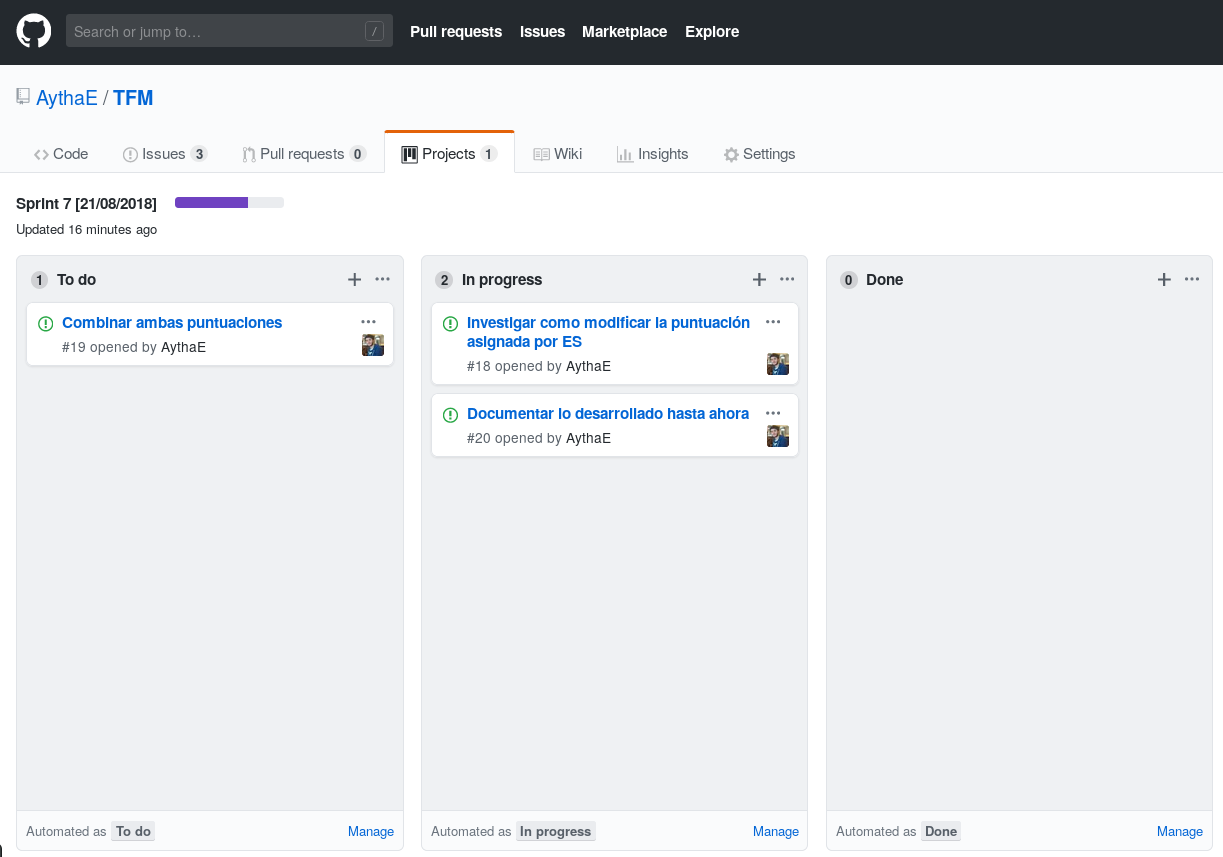
\includegraphics[width=\linewidth]{imagenes/ejemplo_tablero_sprint}
	\caption{Ejemplo de tablero de un \textit{sprint}}
	\label{fig:tableroSprint}
\end{figure}

Además de esto he utilizado un archivo \textit{Markdown} a modo de diario donde ir apuntando cosas interesantes según iban surgiendo, el estado actual de desarrollo o algunas tareas para completar próximamente, dicho fichero se llama \texttt{Diario.md}.

\section{Planificación temporal}

Desde la asignación del \acrshort{TFM}, en diciembre de 2017, me percaté que iba a ser realmente complicado alcanzar la primera convocatoria con la carga de trabajo que suponía el máster. Por lo que decidí tomarlo con calma y llegar a septiembre, pero tras todo finalizar el curso comencé la realización de mis prácticas, lo cual unido a lo extenuado que había acabado el año me impidió alcanzar otra vez el objetivo. 

En Octubre de 2017 comienzo a trabajar, lo cual suponen muchas horas menos al día y me llevo un tiempo adaptarme por lo que no fue hasta Febrero de 2018 cuando me lo empecé a tomar en serio. Teniendo en cuenta mi limitada disponibilidad horaria que apenas me permitía dedicarle 1-2 horas entre diario esbocé una planificación con el objeto de entregar el proyecto en Julio de 2018, dicha planificación inicial se recoge en la siguiente tabla.

\begin{table} [h!]
	\centering
	\begin{tabular}{l c c c}
		\hline
		\textbf{Tarea} & \textbf{Inicio} & \textbf{Fin} & \textbf{Duración}\\
		\hline\hline
		Investigación & 19/02/2018 & 23/04/2018 & 8 semanas \\
		\hline
		Obtención de datos & 23/04/2018 & 07/05/2018 & 2 semanas\\
		\hline
		Procesado de datos & 07/05/2018 & 21/05/2018 & 2 semanas\\
		\hline
		Búsqueda básica & 21/05/2018 & 04/06/2018 & 2 semanas\\
		\hline
		Búsqueda con bibliometría & 04/06/2018 & 02/07/2018 & 4 semanas\\
		\hline
		Refinamiento & 02/07/2018 & 09/07/2018 & 1 semana\\
		\hline
	
	\end{tabular}
	\caption{Planificación inicial de tareas}
\end{table}

Desgraciadamente las vacaciones que he tomado entre medias junto con algunos imprevistos no me permitieron llegar a tiempo aunque ya tenía el proyecto encaminado.

%

%

%
%\input{capitulos/04_Analisis}
%
\chapter{Diseño}


\section{Fuentes de datos}
Al ser este un sistema \acrshort{RI} el diseño ha de girar en torno a los datos, por ello comencé explorando diversas alternativas para utilizar como fuente de datos. 

Como punto inicial para la extracción de los datos de los autores de la \acrshort{ETSIIT} partí del Ranking UGRinvestiga \cite{Ranking_UGRInvestiga}. En este se lista a todos los autores de la escuela junto con sus citas e índice h total y los últimos 5 años.

Sin embargo no hay modo de obtener datos de los artículos concretos por lo que barajé múltiples bases de datos bibliográficas, además de las ya comentadas en la sección \nameref{subsec:sistemasRI} también exploré \href{https://www.researchgate.net/}{Research Gate}.

Los resultados de mi análisis fueron los siguientes: 
\label{ls:dataSourceAnalisis}
\begin{itemize}
	
	\item Google Scholar y Research Gate parecen tener bastantes datos en comparación a otras opciones, sin embargo no ofrecen una \acrshort{API} por lo que la extracción de datos solo se podría llevar a cabo mediante \textit{\gls{webscraping}} \glsrefentry{webscraping}. Esto no es un proceso sencillo, ya que muchas de estas web contienen mecanismos de detección de bots como los CAPTCHAs \cite{scrapping_GS} y además es un método muy sensible al cambio: en caso de que produzca alguna modificación en la web en cuestión es probable que toque reescribir el método de extracción de datos.
	\item \acrshort{WoS} y Scopus sí disponen de una \acrshort{API}, tras realizar algunas pruebas y leer opiniones sobre ambas me decanté por utilizar Scopus como fuente de datos ya que su \acrshort{API} me resultó más cómoda de utilizar y encontré datos fácilmente de algunos autores de la \acrshort{ETSIIT} (cosa que me costó bastante más en \acrshort{WoS}).
\end{itemize}

\section{Modelo de datos}

Siguiendo el modelo de Scopus decidí separar la búsqueda de autores y la de artículos como apunté en los objetivos.

Por tanto mi modelo de datos está constituido por 2 entidades distintas pero relacionadas: Autores (\textit{Author}) y Artículos (\textit{Abstract}). 

En las siguientes secciones se describen brevemente ambas entidades.


\subsection{\textit{Author}}
\label{subsc:author}
Esta entidad es resultado de la combinación de la información disponible en el Ranking UGRinvestiga \cite{Ranking_UGRInvestiga} y en Scopus, por eso podemos ver en el siguiente diagrama con el prefijo \texttt{ugr} las medidas de dicho ranking y con el de \texttt{scopus} los de la plataforma homónima. 

Respecto a los atributos que finalizan en \texttt{5} estos hacen referencia a los valores de dichas medidas de los últimos cinco años.

\begin{figure}[ht]
	
	\centering
	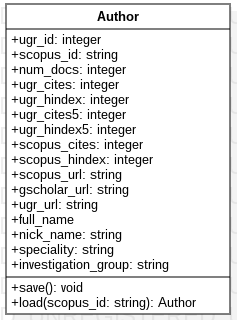
\includegraphics[width=0.5\linewidth]{imagenes/Author}
	\caption{Clase \textit{Author}}
\end{figure}

\newpage

\subsection{\textit{Abstract}}
\label{subsc:abstract}
La entidad \textit{Abstract} corresponde casi directamente con los datos obtenidos a través de la \acrshort{API} de Scopus, a excepción de:
\begin{itemize}
	\item Las referencias han sido limitadas a citas internas, es decir entre los artículos que están disponibles en la colección, con la idea de usar esta información en el proceso de búsqueda.
	\item Los autores, que únicamente aparecían listados con su \texttt{scopus\_id}, han sido enriquecidos con el nombre de los mismos así como el \texttt{ugr\_id} en caso de estar disponible este último (este identificador estará disponible si el autor es alguno de los que forman parte de la colección de autores).
\end{itemize}

\begin{figure}[h]
	
	\centering
	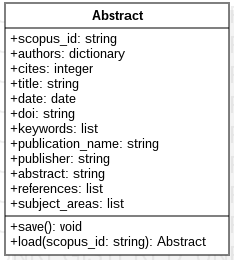
\includegraphics[width=0.5\linewidth]{imagenes/Abstract}
	\caption{Clase \textit{Abstract}}
\end{figure}

\newpage

\section{Arquitectura inicial del sistema}
\label{sc:arq_inicial}
La arquitectura del sistema planteado se basará en el modelo cliente/servidor con tres nodos:
\begin{itemize}
	\item \textbf{Servidor de \acrlong{BD}}: El cual almacenara la información correspondientes a autores y artículos como se ha modelado en el apartado previo.
	\item \textbf{Servidor de \acrshort{RI}}: Donde se llevará a cabo la búsqueda en sí, se servirá del servidor de \acrshort{BD} como almacenamiento de datos y atenderá las peticiones de búsqueda.
	\item \textbf{Cliente}: Parte del sistema que será visible para el usuario y que se encargará de recoger las peticiones de búsqueda, enviarlas al servidor de \acrshort{RI} y presentar los resultados devueltos por el mismo
\end{itemize}

\begin{figure}[ht]
	
	\centering
	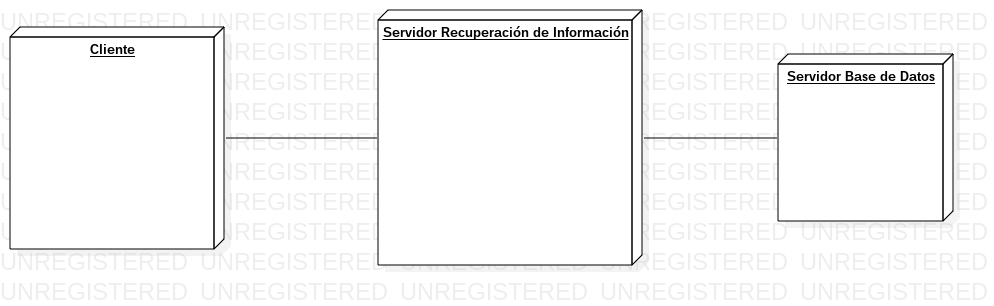
\includegraphics[width=\linewidth]{imagenes/initial_architecture}
	\caption{Diagrama de arquitectura inicial del sistema}

\end{figure}

\chapter{Técnicas y herramientas [Aún en progreso]}
\label{ch:herramientas}

Comentar en más detalle todas las herramientas utilizadas con enlaces de cada una.

\begin{itemize}
	\item \textbf{Debian}: \acrfull{SO}.
	\item \textbf{Python}: Lenguaje de programación usado en las primeras fases del proyecto y en servidor \gls{backend} \glsrefentry{backend}.
	\item \textbf{JavaScript}: Lenguaje de programación interpretado en el que se ha escrito el \gls{frontend} \glsrefentry{frontend}.
	\item \textbf{Elasticsearch}: Servidor de búsqueda.
	\item \textbf{MongoDB}: Base de datos NoSQL.
	\item \textbf{React}:  \Gls{framework} para el desarrollo de interfaces de usuario.
	\item \textbf{Searchkit}: \Gls{framework} que incluye un conjunto de componentes React para la comunicación con Elasticsearch.
	\item \textbf{TeXstudio}: Entorno integrado de escritura en \LaTeX{} utilizado para generación de la documentación.
	\item \textbf{Docker}: Software de virtualización para basado en contenedores. Permite gestionar de forma simple la gestión y despliegue de una infraestructura software.
	\item \textbf{Visual Studio Code}: Editor de código creado por Microsoft utilizado para toda la programación del proyecto.
	\item Git
	\item GitHub
	\item Pandas
	\item PyMongo
	\item scopus-api
	\item Beautiful Soup
	\item Matplotlib
	\item MaterialUI
	\item elasticsearch-py
	\item Star UML
	\item Cerebro
	\item Flask
	\item Gimp
	\item Nginx
	\item uWSGI
\end{itemize}

\chapter{Desarrollo}
En este capítulo se detallara el proceso de desarrollo seguido dividido en \textit{sprints} como ya se ha comentado en la sección \nameref{sc:metodologia}.


\section{\textit{Sprint} 1}
Este primer \textit{sprint} tiene como objetivo general la investigación básica sobre la \acrshort{RI}. Sus objetivos concretos son: 

\begin{itemize}
	\item Leer el libro \acrlong{RI}: un enfoque práctico y multidisplinar \cite{RIspaBook}.
	\item Buscar los talleres \acrshort{BIR} centrándose en sus editoriales para realizar un listado priorizado por interés de los diversos artículos.
\end{itemize}

Siguiendo la recomendación de mi tutor (co-autor del libro) me centré en los capítulos \textit{"1 Introducción a la recuperación de información"}, \textit{"2 Indexación de documentos y procesado de consultas"}, \textit{"3 Modelos de recuperación de información clásicos"} y \textit{"10 Técnicas de modificación de la consulta"}. 

Esta lectura me hizo adquirir unas bases más teóricas a lo que ya había estudiado en la asignatura del máster \acrlong{GIW} donde obtuvimos una nociones básicas de lo que supone la \acrshort{RI} y sus vertientes realizando alguna práctica.

Los artículos de los talleres \acrlong{BIR} que encontré más destacados están detallados en el apartado \nameref{subsc:trabajosRelacionados} de la Introducción. Dichos trabajos se encuentran disponibles gratuitamente en \url{http://ceur-ws.org/} bajo el amparo de la Universidad Técnica de Aquisgrán (\textit{RWTH Aachen University}) en Alemania.

Cada una de las ediciones de estos talleres se encuentra estructurada dividida en diversos trabajos. Por un lado un editorial que resume la edición y todos los trabajos aceptados en la conferencia así como los trabajos individuales, alguna \textit{keynote} o presentación y algunas demostraciones. 

En este \textit{sprint} me dediqué a leer dichos editoriales clasificando por aparente interés los artículos de cada \acrshort{BIR} generando una lista priorizada utilizada como orden en el que estudiar los trabajos. En la siguiente imagen se puede apreciar el aspecto de dicha lista generada en \textit{Markdown}.

\begin{figure}[ht]
	
	\centering
	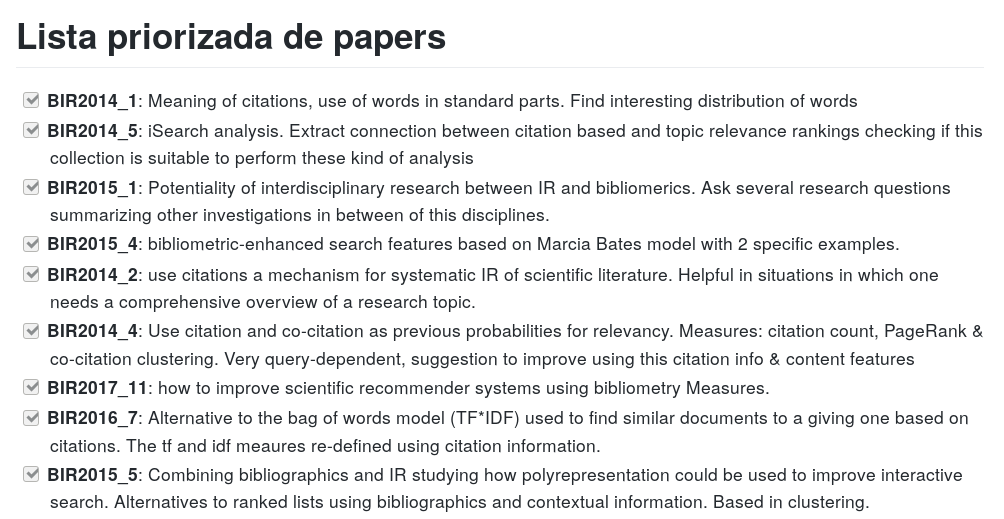
\includegraphics[width=\linewidth]{imagenes/lista_priorizada}
	\caption{Fragmento de la lista priorizada creada}
\end{figure}

\section{\textit{Sprint} 2}
Para el segundo \textit{sprint} plantee el indagar en la \acrshort{RI} e ir introduciendo la bibliometría. Sus objetivos concretos son: 

\begin{itemize}
	\item Leer los primeros 17 papers de los \acrshort{BIR} resumiendo y extrayendo ideas interesantes para el proyecto.
	\item Buscar información sobre medidas bibliométricas (Citas, índice h combinado...)
\end{itemize}

A partir de la lista priorizada fui leyendo los primeros artículos, el orden de esta lista lo fui alterando ya que con frecuencia al indagar en el trabajo este perdía o incrementaba su interés. Con el objetivo de poder aprovechar más estas lecturas fui creando una especie de resúmenes en los que anotaba los puntos más importantes que se trataban en el artículo, otros artículos relacionados de los que se hablaba o los resultados obtenidos con su trabajo. En la siguiente imagen se puede apreciar uno de estos "resúmenes":

\begin{figure}[h!]
	
	\centering
	
\includegraphics[width=\linewidth]{imagenes/paper_sumary}
	\caption{Ejemplo de resumen de uno de los papers}
\end{figure}

En este momento me empecé a introducir en el mundo de las medidas bibliométricas, ya que no tenía conocimiento previo alguno de que existiera esta disciplina siquiera, mediante la lectura de artículos iba descubriendo distintas medidas así como sus posibles aplicaciones a la \acrshort{RI} cuyo resultado final se encuentra sintetizado en la sección \nameref{sc:bibliometria} de la Introducción.

\section{\textit{Sprint} 3}
Ya en este punto decidí que estaba listo para ir documentando todo lo que había aprendido por ello en este \textit{sprint} me puse como objetivo escribir la introducción de este \acrshort{TFM}. Los objetivos concretos son:
\begin{itemize}
	\item Escribir la introducción del \acrshort{TFM}.
	\item Pensar un enfoque para el proyecto a desarrollar decidiendo que clase de sistema se desarrollaría.
	\item Continuar leyendo algunos artículos más de los \acrshort{BIR}.
\end{itemize}

Para asimilar y reflexionar sobre todo lo que había leído me puse a escribir la introducción de este trabajo ya que ello me ayudaría a pensar un enfoque correcto. También quería poder mostrar algo a mi tutor para obtener algo de \textit{feedback} por su parte.

Continué leyendo algunos trabajos más con lo que dí por concluida mi proceso de investigación. Uno de esos últimos trabajos fue \cite{DBLP:conf/ecir/SarolLS18} el cual me gustó especialmente ya que pasaban de un modelo teórico a algo más práctico, accediendo a la \acrshort{API} de Scopus e incluyendo ejemplos de su implementación en un repositorio de \textit{GitHub} lo que me llevo a plantear mi modelo híbrido combinando el sistema habitual de un sistema \acrshort{RI} con reordenamiento de resultados \textit{a priori} usando medidas bibliométricas y un ordenamiento \textit{a posteriori} utilizando un grafo de citación entre los documentos.

Desgraciadamente estos enfoques dependen ampliamente de la cobertura de medidas bibliométricas disponibles, por ejemplo me hubiera encantado poder probar una reordenación previa utilizando alguna \textit{altmetric} como el número de lecturas o descargas de un artículo, pero la plataforma que he utilizado para extraer los artículos no dispone de dichas medidas.

Como parte adicional de este sprint también estuve haciendo alguna pruebas con \glspl{framework} de búsqueda. Como he dicho previamente ya había utilizado \textit{Lucene} como parte de las prácticas de la asignatura \acrshort{GIW}, pero me pareció demasiado bajo nivel así que me centré en investigar otras alternativas. Encontré que las principales, que casualmente utilizaban por debajo \textit{Lucene}, eran \textit{\textbf{Solr}} y \textit{\textbf{\acrlong{ES}}}.

Buscando alguna comparativa \cite{ES_Solr} y comentarios de usuarios en plataformas tan reputadas como \textit{StackOverflow} \cite{ES_Solr_SO} parecía que se recomendaba \acrshort{ES} por ser más sencillo de usar por lo que realicé un breve tutorial \cite{ES_tutorial} que me gustó bastante ya que resulta realmente simple de usar y basta únicamente con realizar consultas sobre una \acrshort{API} \acrshort{REST} por lo que basta con hacer peticiones \acrshort{HTTP} con algún cliente simple como \texttt{curl}. Todo esto hizo que me decidiera por este servidor de búsqueda.


\section{\textit{Sprint} 4}

\section{\textit{Sprint} 5}

\section{\textit{Sprint} 6}

\section{\textit{Sprint} 7}

\section{\textit{Sprint} 8}
%
%\input{capitulos/06_Implementacion}
%
%\input{capitulos/07_Pruebas}
%
\chapter{Conclusiones y Trabajos Futuros}

\section{Relación del \acrshort{TFM} con lo aprendido en el Máster}

GIW

SSBW

CC


\section{Conclusiones}

Proyecto interesante

Curiosidad planteada en la motivacion satisfecha

No tiempo suficiente para llevar a cabo todo lo planteado. Objetivo de  Evaluación no cumplido

\section{Trabajos futuros}
Relevance feedback

Redes de citación

Intentar obtener Altmetrics de otras fuentes

\textbf{Evaluar la mejora producida al aplicar medidas bibliométricas al sistema}: como colección de datos del sistema \acrshort{RI} a desarrollar se ha decidido utilizar el conjunto de todos los trabajos de autores de la \myFaculty lo que favorece que esta evaluación se pueda llevar a cabo, aunque esta no es una tarea sencilla. La evaluación de sistemas \acrshort{RI} se suele llevar a cabo mediante colecciones de prueba donde existe un conjunto de documentos, un conjunto de consultas y un conjunto de resultados que deberían de retornar las mismas  \cite{RI_Evaluation}. Al crear un sistema nuevo con una colección de documentos no utilizada no podemos comparar los resultados obtenidos con los que se esperarían, este problema se debe a la relatividad del concepto de relevancia. Por ello las colecciones de pruebas suelen incluir valoraciones de relevancia de expertos en la materia.
%
%%\chapter{Conclusiones y Trabajos Futuros}
%
%
%\nocite{*}
\bibliographystyle{ieeetr}
\bibliography{bibliografia/bibliografia} \addcontentsline{toc}{chapter}{Bibliografía}

\appendix
\clearpage
\addappheadtotoc
\appendixpage

%%\input{apendices/paper/paper}



\printnoidxglossary[sort=use]
%\addcontentsline{toc}{chapter}{Glosario}

\printnoidxglossary[type=\acronymtype, title=Lista de Acrónimos]
%\addcontentsline{toc}{chapter}{Lista de Acrónimos}
\chapter{Manual técnico de uso}

\section{Descripción de la arquitectura}
El sistema desarrollado a lo largo de este proyecto se ha servido de \textit{Docker} como forma de gestionar la infraestructura de los diversos nodos que lo conforman. La arquitectura final del sistema como se recoge en la figura \ref{fig:finalArchitecture} se constituye de 4 nodos o contenedores \textit{Docker} concretamente.

\begin{itemize}
	\item \textit{\textbf{app}}: contenedor que contiene una imagen con un servidor \textit{Nginx} encargado de servir el \gls{frontend} \textit{React} y el cual se comunica con servidor de aplicación \textit{uWSGI} mediante un \textit{socket UNIX}. Dicho servidor de aplicación sirve la aplicación \textit{Flask} que constituye el \gls{backend} del sistema.
	\item \textit{\textbf{elasticsearch}}: contenedor en el cual se encuentra alojada una imagen de \acrlong{ES} en su versión \textit{Open Source} siguiendo las instrucciones oficiales \cite{ES_docker}.
	\item \textit{\textbf{mongodb}}: contenedor con la imagen de \textit{MongoDB} utilizada
	\item \textit{\textbf{cerebro}}: contenedor con el servicio de monitorización de \acrshort{ES} \textit{Cerebro}. Este contenedor no es necesario para el funcionamiento del sistema pero ha resultado muy útil durante el desarrollo para gestionar el contenedor de \acrshort{ES}
\end{itemize}

\section{\texttt{docker-compose.yml}}
En el siguiente listing se observa la configuración del fichero \texttt{docker-compose.yml} que determina la infraestructura descrita arriba.

\lstinputlisting[language=yaml, caption=Fichero \texttt{docker-compose.yml} de la aplicación]{code/docker-compose.yml}

\section{Instalación}
\subsection{Docker y Docker Compose}
Para poder desplegar la aplicación por tanto lo primero sera instalar \textit{Docker} y \textit{Docker Compose}. Para instalar \textit{Docker} se ha utilizado su versión \textit{Community Edition (CE)} por ello ver las instrucciones de instalación para el sistema en el que se desee instalar \cite{dockerInstall}. Respecto a \textit{Docker Compose} recomiendo instalar la versión nativa para el sistema de destino en lugar de utilizar las opciones alternativas de instalación, ver la documentación oficial en \cite{dockerComposeInstall}.

\newpage

\subsection{Descripción del repositorio}
Una vez instalado esto sera necesario \textit{clonar} el repositorio de \textit{GitHub}, que recuerdo era \url{https://github.com/AythaE/TFM}, cuya estructura se observa a continuación. Para disponer de los datos de \textit{MongoDB} y \acrlong{ES} será necesario descomprimir el fichero \texttt{data.7z}. Esto creara una carpeta \texttt{data}.

\dirtree{%
.1 TFM.
.2 data/.
.3 es\_data/.
.3 mongodb\_data/.
.2 config/.
.3 elasticsearch.yml.
.2 src/.
.3 backend/\DTcomment{Código \gls{backend} y fichero \texttt{requirements.txt} con las dependencias de \textit{Python}}.
.3 frontend/\DTcomment{Código \gls{frontend} y fichero \texttt{package.json} con las dependencias de \textit{JS}}.
.3 Exploring/.
.4 elasticsearch/\DTcomment{Código de indexación en \acrshort{ES}}.
.4 Exploratory\_analysis/\DTcomment{Ficheros y gráficos generados en el análisis de datos}.
.4 investigadores/\DTcomment{Código extracción de datos del ranking UGRinvestiga}.
.4 scopus/\DTcomment{Código extracción de datos de Scopus}.
.3 Dockerfile\DTcomment{Fichero que dertermina la construcción del contenedor \textit{\textbf{app}}}.
.2 docker-compose.yml.
}

\section{Despliegue}
Con todo esto ya estamos listos para desplegar la aplicación. Para ello basta con ejecutar el siguiente comando desde el directorio \texttt{TFM}:

\begin{lstlisting}[style=Consola, caption=Comando para desplegar el sistema]
$ docker-compose -f "docker-compose.yml" up --build
\end{lstlisting}

Una vez finalice la construcción del contenedor \textbf{\textit{app}} se mostrarán unos mensajes indicando que todos los contenedores han arrancado correctamente, tras esto podremos acceder a \url{http://localhost} donde se encontrará desplegada la aplicación.

En caso de algún problema en el despliegue esto seguramente se deba a los puertos disponibles, el sistema utiliza los puertos 80 (acceso \acrshort{HTTP} \gls{frontend}), 27017 (\textit{MongoDB}), 9000 (\textit{Cerebro}), 9200 y 9300 (\acrlong{ES}). Por lo que si alguno de esos puertos se encuentra en uso el despliegue fallará. Dicho mapeo de puertos se puede cambiar fácilmente modificando los \texttt{ports} en el fichero \texttt{docker-compose.yml}.


Para parar la aplicación basta con aplicar un \texttt{Ctrl\^\ C} sobre la consola donde se esté ejecutando el comando de despliegue.




\chapter*{}
\thispagestyle{empty}

\end{document}
